
\documentclass[11pt]{article}
\usepackage[a4paper,margin=1in]{geometry}
\usepackage{amsmath,amssymb}
\usepackage{graphicx}
\usepackage[dvipsnames]{xcolor}
\usepackage{hyperref}
\usepackage{enumitem}
\usepackage{tabularx}
\usepackage{longtable}
\usepackage{booktabs}
\usepackage[most]{tcolorbox}
\usepackage{titlesec}
\usepackage{xurl}
\usepackage{fancyhdr}
\usepackage{setspace}
\usepackage{tikz}
\usetikzlibrary{positioning,arrows.meta}
\usepackage[T1]{fontenc}
\usepackage{lmodern}
\setlength{\parindent}{0pt}
\setlength{\parskip}{8pt}
\setlength{\headheight}{14pt}
\setstretch{1.12}
\setlist[itemize]{leftmargin=1.5em, nosep}
\setlist[enumerate]{leftmargin=1.5em, nosep}
\providecommand{\tightlist}{\setlength{\itemsep}{0pt}\setlength{\parskip}{0pt}}
\hypersetup{colorlinks=true,linkcolor=MidnightBlue,urlcolor=MidnightBlue}
\pagestyle{fancy}
\fancyhf{}
\rhead{\thepage}
\renewcommand{\headrulewidth}{0pt}
\renewcommand{\footrulewidth}{0pt}
\titleformat{\section}{\Large\bfseries\color{MidnightBlue}}{\thesection}{0.6em}{}
\titleformat{\subsection}{\bfseries}{}{0em}{}


\begin{document}

\begin{center}\LARGE\bfseries KG Foundations: Provenance, Maintenance, and Context Pipeline\end{center}

\begin{center}\large Block 3 Day 3\end{center}

\begin{tcolorbox}[colback=MidnightBlue!4,colframe=MidnightBlue,title={Session Overview},fonttitle=\bfseries,breakable]
\textbf{Session objective:} Build trustworthy knowledge-graph reasoning pipelines using provenance, entity resolution, freshness, and context selection.

\textbf{Timing target (min):} 71

\textbf{Topic anchors:} knowledge graph; schema; instance; provenance; entity resolution; freshness; context pipeline

\textbf{Padlet board:} \url{https://padlet.com/qmul/b3-d3-ap6e0bmcfc9tuhlx}
\end{tcolorbox}

\section*{Exercises}

\begin{tcolorbox}[colback=white,colframe=MidnightBlue,title={Q1 Core Concept Check},fonttitle=\bfseries,breakable]
\begin{center}
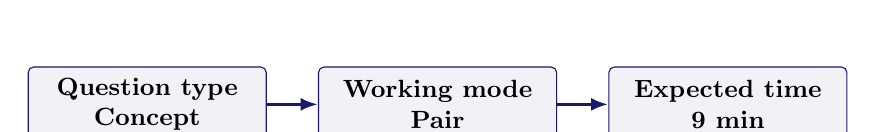
\begin{tikzpicture}[
node distance=0.65cm,
box/.style={draw=MidnightBlue, rounded corners=2pt, minimum height=0.95cm, align=center, font=\small\bfseries, fill=MidnightBlue!6, text width=0.23\linewidth},
arrow/.style={-{Latex[length=2.2mm]}, very thick, MidnightBlue}
]
\node[box] (type) {Question type\\Concept};
\node[box, right=of type] (mode) {Working mode\\Pair};
\node[box, right=of mode] (time) {Expected time\\9 min};
\draw[arrow] (type) -- (mode);
\draw[arrow] (mode) -- (time);
\end{tikzpicture}
\end{center}

{\large\bfseries\color{MidnightBlue} Prompt}\par\medskip
Classify each statement as schema or instance, then rewrite one statement that is wrongly expressed. Statements: (1) Module taughtBy Lecturer, (2) EBU6505 taughtBy Dr\_Riasat\_Islam, (3) Room locatedIn Building, (4) Lecturer isIn Mile\_End\_Campus. Treat statement (4) as badly written and repair it so that it becomes a clearer graph fact or graph pattern.

{\large\bfseries\color{MidnightBlue} Task details}\par\medskip
\begin{itemize}\item \textbf{Type:} concept
\item \textbf{Mode:} pair
\item \textbf{Time:} 9 min
\item \textbf{Deliverable:} classification + repair
\item \textbf{Assessment focus:} distinguish schema structure from instance facts and detect mixed-up graph statements
\item \textbf{Expected length:} 4 labels + 1 correction\end{itemize}

{\large\bfseries\color{MidnightBlue} How to submit}\par\medskip
Post one pair Padlet comment with four labels and one corrected statement.

{\large\bfseries\color{MidnightBlue} Discussion in class}\par\medskip
Which clue tells you fastest that a statement is a pattern rather than a stored fact?

{\large\bfseries\color{MidnightBlue} Why this helps}\par\medskip
Useful for graph-structure questions that ask students to separate graph design from graph data.

{\large\bfseries\color{MidnightBlue} References}\par\medskip
\begin{itemize}\item Russell \& Norvig (2021) AIMA 4e, Ch.10, pp.314-343
\item Poole \& Mackworth (2023) 3e, Ch.16, pp.701-730 and Ch.17, pp.731-766\end{itemize}
\end{tcolorbox}

\begin{tcolorbox}[colback=white,colframe=MidnightBlue,title={Q2 Structured Problem},fonttitle=\bfseries,breakable]
\begin{center}
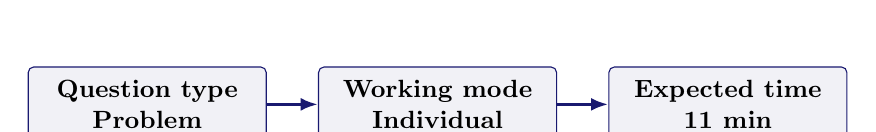
\begin{tikzpicture}[
node distance=0.65cm,
box/.style={draw=MidnightBlue, rounded corners=2pt, minimum height=0.95cm, align=center, font=\small\bfseries, fill=MidnightBlue!6, text width=0.23\linewidth},
arrow/.style={-{Latex[length=2.2mm]}, very thick, MidnightBlue}
]
\node[box] (type) {Question type\\Problem};
\node[box, right=of type] (mode) {Working mode\\Individual};
\node[box, right=of mode] (time) {Expected time\\11 min};
\draw[arrow] (type) -- (mode);
\draw[arrow] (mode) -- (time);
\end{tikzpicture}
\end{center}

{\large\bfseries\color{MidnightBlue} Prompt}\par\medskip
Given the triples EBU6505 taughtBy Dr\_Riasat\_Islam, Dr\_Riasat\_Islam officeRoom TB\_3\_335, TB\_3\_335 locatedIn Engineering\_Building, and Engineering\_Building onCampus Mile\_End, answer the question Where can a student go for EBU6505 lecturer support? State the graph path you use and one caveat about the answer.

{\large\bfseries\color{MidnightBlue} Task details}\par\medskip
\begin{itemize}\item \textbf{Type:} problem
\item \textbf{Mode:} individual
\item \textbf{Time:} 11 min
\item \textbf{Deliverable:} path reasoning result
\item \textbf{Assessment focus:} follow a multi-hop graph path and state a justified conclusion
\item \textbf{Expected length:} 1 path + 1 answer + 1 caveat\end{itemize}

{\large\bfseries\color{MidnightBlue} How to submit}\par\medskip
Post your own Padlet comment with the path, the answer, and one confidence caveat.

{\large\bfseries\color{MidnightBlue} Discussion in class}\par\medskip
At which step does the answer become less certain?

{\large\bfseries\color{MidnightBlue} Why this helps}\par\medskip
Direct practice for multi-hop reasoning and evidence-based conclusions.

{\large\bfseries\color{MidnightBlue} References}\par\medskip
\begin{itemize}\item Russell \& Norvig (2021) AIMA 4e, Ch.10, pp.314-343
\item Poole \& Mackworth (2023) 3e, Ch.16, pp.701-730 and Ch.17, pp.731-766\end{itemize}
\end{tcolorbox}

\begin{tcolorbox}[colback=white,colframe=MidnightBlue,title={Q3 Structured Problem},fonttitle=\bfseries,breakable]
\begin{center}
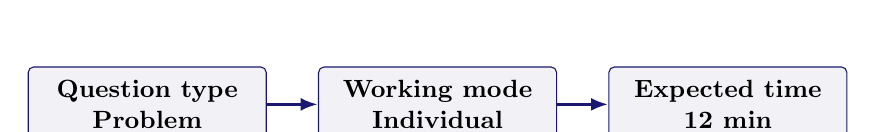
\begin{tikzpicture}[
node distance=0.65cm,
box/.style={draw=MidnightBlue, rounded corners=2pt, minimum height=0.95cm, align=center, font=\small\bfseries, fill=MidnightBlue!6, text width=0.23\linewidth},
arrow/.style={-{Latex[length=2.2mm]}, very thick, MidnightBlue}
]
\node[box] (type) {Question type\\Problem};
\node[box, right=of type] (mode) {Working mode\\Individual};
\node[box, right=of mode] (time) {Expected time\\12 min};
\draw[arrow] (type) -- (mode);
\draw[arrow] (mode) -- (time);
\end{tikzpicture}
\end{center}

{\large\bfseries\color{MidnightBlue} Prompt}\par\medskip
A graph stores two room facts for the same lecturer: one came from an official timetable export yesterday, and one came from an anonymous note posted three months ago. Decide which fact should be trusted more, what provenance should be stored with it, and whether the older fact should be deleted, flagged, or kept.

{\large\bfseries\color{MidnightBlue} Task details}\par\medskip
\begin{itemize}\item \textbf{Type:} problem
\item \textbf{Mode:} individual
\item \textbf{Time:} 12 min
\item \textbf{Deliverable:} provenance judgement
\item \textbf{Assessment focus:} compare evidence quality using provenance and freshness
\item \textbf{Expected length:} 3 short decisions\end{itemize}

{\large\bfseries\color{MidnightBlue} How to submit}\par\medskip
Post your own Padlet comment with three short decisions and one reason for each.

{\large\bfseries\color{MidnightBlue} Discussion in class}\par\medskip
Is a recent source always enough, or does source authority still matter?

{\large\bfseries\color{MidnightBlue} Why this helps}\par\medskip
Useful for questions about provenance, trust, and freshness in graph-backed agents.

{\large\bfseries\color{MidnightBlue} References}\par\medskip
\begin{itemize}\item Russell \& Norvig (2021) AIMA 4e, Ch.10, pp.314-343
\item Poole \& Mackworth (2023) 3e, Ch.16, pp.701-730 and Ch.17, pp.731-766\end{itemize}
\end{tcolorbox}

\begin{tcolorbox}[colback=white,colframe=MidnightBlue,title={Q4 Stretch Extension},fonttitle=\bfseries,breakable]
\begin{center}
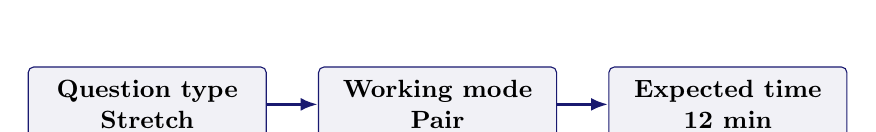
\begin{tikzpicture}[
node distance=0.65cm,
box/.style={draw=MidnightBlue, rounded corners=2pt, minimum height=0.95cm, align=center, font=\small\bfseries, fill=MidnightBlue!6, text width=0.23\linewidth},
arrow/.style={-{Latex[length=2.2mm]}, very thick, MidnightBlue}
]
\node[box] (type) {Question type\\Stretch};
\node[box, right=of type] (mode) {Working mode\\Pair};
\node[box, right=of mode] (time) {Expected time\\12 min};
\draw[arrow] (type) -- (mode);
\draw[arrow] (mode) -- (time);
\end{tikzpicture}
\end{center}

{\large\bfseries\color{MidnightBlue} Prompt}\par\medskip
You have a 600-token context budget. Create an evidence-packet strategy for a campus assistant answering: Where is today's class and who can I contact if it changes? State what must be included, what can be left out, and why.

{\large\bfseries\color{MidnightBlue} Task details}\par\medskip
\begin{itemize}\item \textbf{Type:} stretch
\item \textbf{Mode:} pair
\item \textbf{Time:} 12 min
\item \textbf{Deliverable:} context-budget plan
\item \textbf{Assessment focus:} compress graph evidence into a small retrieval packet
\item \textbf{Expected length:} 5 bullets\end{itemize}

{\large\bfseries\color{MidnightBlue} How to submit}\par\medskip
Post one pair Padlet comment with five bullets covering essential evidence, optional evidence, and one item you would drop first if the budget shrinks.

{\large\bfseries\color{MidnightBlue} Discussion in class}\par\medskip
Which evidence item should never be removed, even under a very small budget?

{\large\bfseries\color{MidnightBlue} Why this helps}\par\medskip
Good extension for questions on retrieval budgets, evidence selection, and context management.

{\large\bfseries\color{MidnightBlue} References}\par\medskip
\begin{itemize}\item Russell \& Norvig (2021) AIMA 4e, Ch.10, pp.314-343
\item Poole \& Mackworth (2023) 3e, Ch.16, pp.701-730 and Ch.17, pp.731-766
\item doi:10.1109/TNNLS.2024.3420218
\item doi:10.1016/j.iswa.2025.200541\end{itemize}
\end{tcolorbox}

\begin{tcolorbox}[colback=white,colframe=MidnightBlue,title={Q5 Collaborative Mini-Case},fonttitle=\bfseries,breakable]
\begin{center}
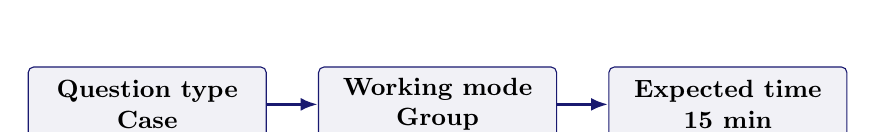
\begin{tikzpicture}[
node distance=0.65cm,
box/.style={draw=MidnightBlue, rounded corners=2pt, minimum height=0.95cm, align=center, font=\small\bfseries, fill=MidnightBlue!6, text width=0.23\linewidth},
arrow/.style={-{Latex[length=2.2mm]}, very thick, MidnightBlue}
]
\node[box] (type) {Question type\\Case};
\node[box, right=of type] (mode) {Working mode\\Group};
\node[box, right=of mode] (time) {Expected time\\15 min};
\draw[arrow] (type) -- (mode);
\draw[arrow] (mode) -- (time);
\end{tikzpicture}
\end{center}

{\large\bfseries\color{MidnightBlue} Prompt}\par\medskip
Design a weekly knowledge-graph maintenance workflow for a campus assistant. Your workflow must include ingestion, entity resolution, provenance capture, freshness checks, validation, and publication.

{\large\bfseries\color{MidnightBlue} Task details}\par\medskip
\begin{itemize}\item \textbf{Type:} case
\item \textbf{Mode:} group
\item \textbf{Time:} 15 min
\item \textbf{Deliverable:} maintenance workflow
\item \textbf{Assessment focus:} design a KG maintenance pipeline with trust controls
\item \textbf{Expected length:} 6 steps + role labels\end{itemize}

{\large\bfseries\color{MidnightBlue} How to submit}\par\medskip
Post one group Padlet comment with a numbered six-step workflow and say who or what checks each step.

{\large\bfseries\color{MidnightBlue} Discussion in class}\par\medskip
Which maintenance step prevents the biggest future reasoning error?

{\large\bfseries\color{MidnightBlue} Why this helps}\par\medskip
Supports case questions on how to keep a graph trustworthy after initial ingestion.

{\large\bfseries\color{MidnightBlue} References}\par\medskip
\begin{itemize}\item Russell \& Norvig (2021) AIMA 4e, Ch.10, pp.314-343
\item Poole \& Mackworth (2023) 3e, Ch.16, pp.701-730 and Ch.17, pp.731-766\end{itemize}
\end{tcolorbox}

\begin{tcolorbox}[colback=white,colframe=MidnightBlue,title={Q6 Exam-Style Constructed Response},fonttitle=\bfseries,breakable]
\begin{center}
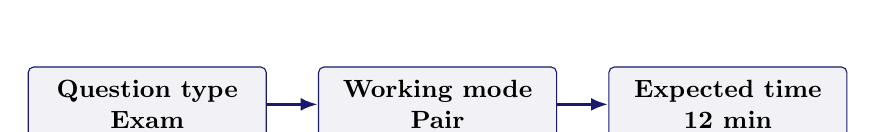
\begin{tikzpicture}[
node distance=0.65cm,
box/.style={draw=MidnightBlue, rounded corners=2pt, minimum height=0.95cm, align=center, font=\small\bfseries, fill=MidnightBlue!6, text width=0.23\linewidth},
arrow/.style={-{Latex[length=2.2mm]}, very thick, MidnightBlue}
]
\node[box] (type) {Question type\\Exam};
\node[box, right=of type] (mode) {Working mode\\Pair};
\node[box, right=of mode] (time) {Expected time\\12 min};
\draw[arrow] (type) -- (mode);
\draw[arrow] (mode) -- (time);
\end{tikzpicture}
\end{center}

{\large\bfseries\color{MidnightBlue} Prompt}\par\medskip
A student asks for the lecturer's office hour. The graph contains two conflicting facts: one from the official module page updated this morning, and one from an old departmental PDF uploaded six months ago. Explain how the agent should resolve the conflict using provenance, freshness, and source authority. Then say what the agent should do if the conflict cannot be resolved automatically.

{\large\bfseries\color{MidnightBlue} Task details}\par\medskip
\begin{itemize}\item \textbf{Type:} exam
\item \textbf{Mode:} pair
\item \textbf{Time:} 12 min
\item \textbf{Deliverable:} structured response
\item \textbf{Assessment focus:} resolve conflicting graph evidence using provenance, freshness, and source authority
\item \textbf{Expected length:} 180-240 words\end{itemize}

{\large\bfseries\color{MidnightBlue} How to submit}\par\medskip
Post one pair Padlet comment with a recommendation, two reasons, and one fallback action for unresolved conflict.

{\large\bfseries\color{MidnightBlue} Discussion in class}\par\medskip
If freshness and authority disagree, which one should dominate first?

{\large\bfseries\color{MidnightBlue} Why this helps}\par\medskip
Matches longer questions on evidence conflict, grounded answers, and trustworthy graph retrieval.

{\large\bfseries\color{MidnightBlue} References}\par\medskip
\begin{itemize}\item Russell \& Norvig (2021) AIMA 4e, Ch.10, pp.314-343
\item Poole \& Mackworth (2023) 3e, Ch.16, pp.701-730 and Ch.17, pp.731-766
\item doi:10.1109/TNNLS.2024.3420218
\item doi:10.1016/j.iswa.2025.200541\end{itemize}
\end{tcolorbox}

\section*{Submission Instructions}

Use the seeded Padlet posts for Q1--Q6. Q2 and Q3 are individual. Q1, Q4, and Q6 are pair tasks. Q5 should be one joint group comment. Start each comment with your names or group label.

\section*{Whole-Class Debrief Prompts}

\begin{itemize}
\tightlist
\item
  Which graph path gave the strongest answer, and where did uncertainty enter?
\item
  What is the difference between keeping a graph fresh and keeping it trustworthy?
\item
  What evidence should never be dropped from a small context packet?
\end{itemize}

\section*{Exam Transfer Note (Day-Level)}

Maps to exam questions on schema versus instance, multi-hop reasoning, provenance, freshness, maintenance workflows, and evidence selection for graph-backed agents.

\end{document}
